% !TEX root = ../Thesis.tex
\chapter{Background}

%This is the body of the thesis.

%\section{Section}
%\label{sec:mylabel}

%\subsection{Sub-Section}

%\subsubsection{Sub-Sub-Section}

%\paragraph{Paragraph}

%\subparagraph{Even Sub-Paragraph}

%Testt This is the body text. Make sure that when you reference anything you use labels and references. When you refer to anything, you normally capitalise the type of object you reference~\ref{sec:mylabel} to, e.g. Section~\ref{sec:mylabel} instead of section~\ref{sec:mylabel}. You may also just use the \texttt{cref} command and it will generate the label, e.g., for \cref{sec:mylabel}, we did not specify the word ``Section''.

%Hint: Try to structure your labels as it is done with \texttt{sec:my-label} and \texttt{fig:machine}, etc.

%A Turing Machine is a 7-Tuple:
%\begin{equation}
    %M = \langle Q, \Gamma, b, \Sigma, \delta, q_0, F \rangle
%\end{equation}
%A Turing Machine is a 7-Tuple even if defined in the text, as in $M = \langle Q, \Gamma, b, \Sigma, \delta, q_0, F \rangle$.

\section{Long Range (LoRa) Wireless Technology}
\label{sec:lora}
In recent years the number of devices connected to the Internet of Things (IoT) has been increasing rapidly. Since a lot of those devices do not need to transfer high amounts of data and rather focus on using as little energy as possible, LoRa and similar technologies have been developed to serve those use-cases. In this section we will give a short overview of how LoRa works and how we can adjust its parameters. \\
LoRa promises long battery life, far-reaching communication distances (10 to 15 kilometres if devices are in line-of-sight) and high node density (nodes in close proximity can operate at the same time if configured correctly). The downside of having all those practical features is a lower data rate. To achieve this, it uses chirp spread spectrum modulation. Data that has to be sent is converted into \textit{upchirps} and \textit{downchirps}. Chirping up or down refers to a signal that is sent with constantly increasing or decreasing frequency. To adjust the transmission settings optimally to specific environments, different parameters that alter the chirps can be configured individually. One of those parameter is the \textbf{bandwidth}. The bandwidth is the difference in frequency of the start and end of one chirp and is typically set to 125, 250 or 500kHz. A higher bandwidth increases the acceptable transmission distance. Another parameter is the \textbf{spreading factor}. It determines the angle of one chirp. The higher the spreading factor, the longer it takes to complete one chirp. This can increase the transmission distance but reduces the data rate. Additionally to the physical settings we can set different \textbf{coding rates} which determine the forward error correction. A higher coding rate leads to a more reliable reception of packets and a lower data rate.
For our project we use a spreading factor of 7, bandwidth of 250kHz and a coding rate of 4/7. These settings have worked well to test the software but need to be reconsidered once the devices get deployed depending on the surrounding conditions.
\begin{figure}
\centering
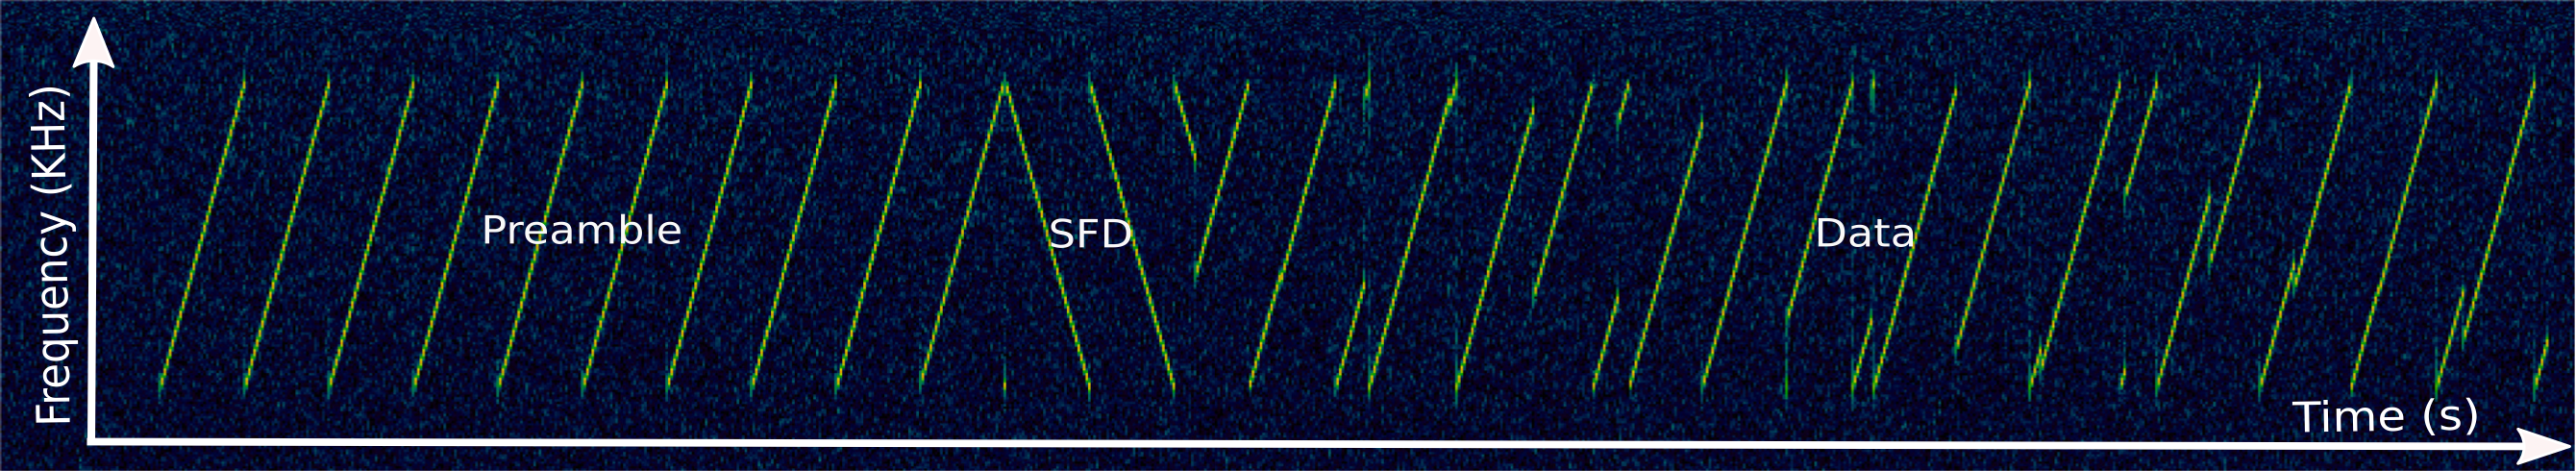
\includegraphics[width=1\textwidth]{chirps}
\caption{A visualized lora packet transmission. Source:~\cite{10.1145/3293534}}
\label{fig:chirps}
\end{figure} \\
In \cref{fig:chirps} we can see ten upchirps (preamble) and two downchirps (start frame delimiter) followed by modulated chirps that contain the actual data. 

(Sources for \cref{sec:lora} are~\cite{10.1007/978-3-030-01168-0_11} and~\cite{10.1145/3293534})

\section{Comparing SSB and TinySSB}

\subsection{SSB}



\subsection{TinySSB}

\section{Pycom 4}




%\section{Tables}
%Some tables can also be used as shown in \cref{tab:table}\footnote{Table captions are normally above the table.}. Remember that tables might be positioned elsewhere in the document. You can force positioning by putting a \texttt{ht!} in the definition.

%\begin{table}[ht!]
%\centering
%\caption{Frequency of Paper Citations. By the way: Make sure to put the label always after the caption, otherwise \LaTeX{} might reference wrongly!}
%\begin{tabular}{lcl} \toprule
%Title&$f$&Comments\\ \midrule
%The chemical basis of morphogenesis & 7327 & \\ 
%On computable numbers, with an application to the ... & 6347 & Turing Machine\\
%Computing machinery and intelligence & 6130 & \\ \bottomrule
%\end{tabular}
%\label{tab:table}
%\end{table}




%\section{Figures}
%Figures are nice to show concepts visually. For organising well your thesis, put all figures in the Figures folder. Figure~\ref{fig:machine} shows how to insert an image into your document. \Cref{fig:tm} references a figure with multiple sub-figures, whereas the sub-figures are referenced by \cref{fig:tm:tm1}, etc. \todoMissing{Description of figure.}

%\begin{figure}
%\centering
%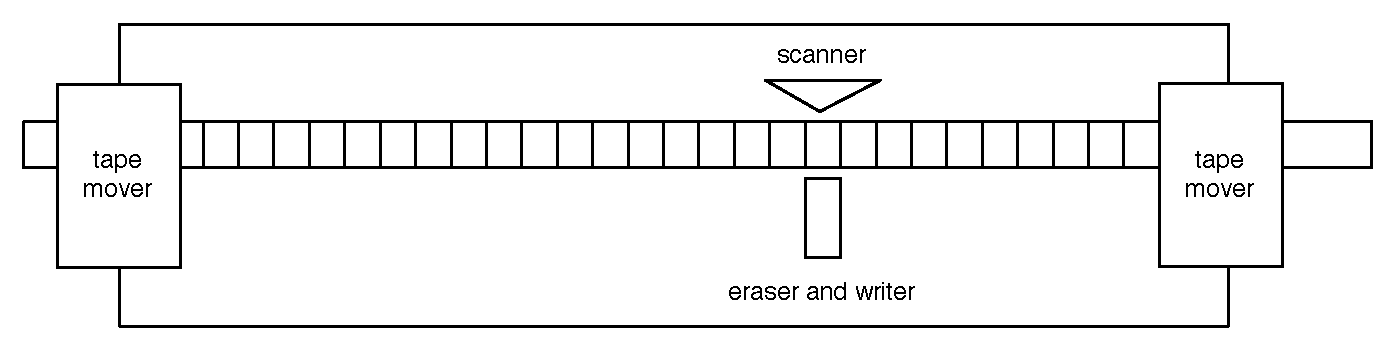
\includegraphics[width=0.9\textwidth]{turingmachine}
%\caption{A Turing machine.}
%\label{fig:machine}
%\end{figure}


%\begin{figure}
%\centering
%\subbottom[Turing Machine 1\label{fig:tm:tm1}]{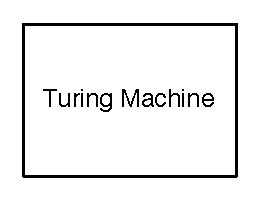
\includegraphics[width=0.2\textwidth]{block}}
%\subbottom[Turing Machine 2\label{fig:tm:tm2}]{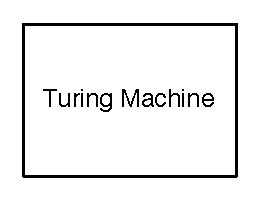
\includegraphics[width=0.2\textwidth]{block}}
%\subbottom[Turing Machine 3\label{fig:tm:tm3}]{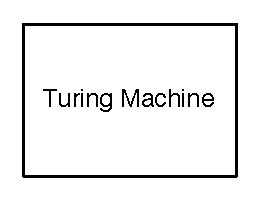
\includegraphics[width=0.2\textwidth]{block}}
%\subbottom[Turing Machine 4\label{fig:tm:tm4}]{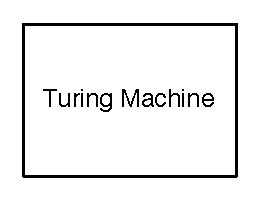
\includegraphics[width=0.2\textwidth]{block}}
%\caption{Plots of four Turing machines}
%\label{fig:tm}
%\end{figure}




\section{Packages}
These packages might be helpful for writing your thesis:

\begin{description}
	\item[\texttt{caption}] to adjust the look of your captions
	\item[\texttt{glossaries}] for creating glossaries (also list of symbols)
	\item[\texttt{makeidx}] for indexes and the back of your document
	\item[\texttt{algorithm, algorithmicx, algpseudocode}] for adding algorithms to your document
\end{description}